\chapter{Permutations}
Recall that permutation is a bijection from $[n]$ to $[n]$. We already discussed
several properties of them. In this chapter we will discuss some combinatorial
properties of them. We denote by $S_n$ the set of all permuations of
$[n]$.\footnote{%
  Letter $S$ is used since in the group theory this set is called
  the symmetric group.
}
\nomenclature[S]{$S_n$}{denote the set of all permuations of $[n]$}


The main operation over permutations is composition, for two permutations $p$
and $q$ we denote their composition $p \circ q$ by $pq$.\footnote{%
  Some authors dentoe $q \circ p$ by $pq$.
}
Note that this operation is not commutative; i.e. $p \circ q$ is not
necessarily equal to $q \circ p$.

Every permutation $p$ can is uniquely detemined by the values $p(1)$, \dots,
$p(n)$, thus sometimes we denote the permutation $f$ by a seqence
$p(1) p(2) \dots p(n)$ (we call it \emph{one-line notation}).
For example, the permutation $3 1 2$ is equal to the function $p : [3] \to [3]$
such that
\[
  p(x) =
  \begin{cases}
    3 & \text{if } x = 1 \\
    1 & \text{if } x = 2 \\
    2 & \text{if } x = 3
  \end{cases}.
\]


\section{Cycles}
Consider the permutation $p$ equal to $2 3 1 5 4$ and draw a digram with
$5$ points where we draw an arrow from $i$ to $j$ iff $p(i) = j$.
\begin{center}
  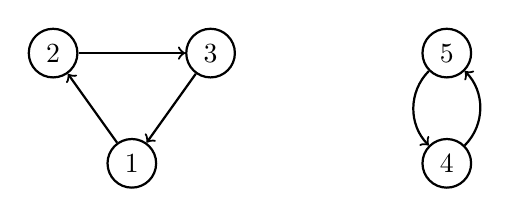
\begin{tikzpicture}[thick]%
    \node[circle, draw, minimum width=4pt]
      (p1) at (0, 0) {1};
    \node[circle, draw, minimum width=4pt]
      (p2) at (-1, 1.4) {2};
    \node[circle, draw, minimum width=4pt]
      (p3) at (1, 1.4) {3};
    \node[circle, draw, minimum width=4pt]
      (p4) at (4, 0) {4};
    \node[circle, draw, minimum width=4pt]
      (p5) at (4, 1.4) {5};
    \draw[->] (p1) -- (p2);
    \draw[->] (p2) -- (p3);
    \draw[->] (p3) -- (p1);

    \draw[->] (p4) to[out=45, in=-45] (p5);
    \draw[->] (p5) to[out=-135, in=135] (p4);
  \end{tikzpicture}
\end{center}
It is easy to see that there are two ``cycles'' in the diagram. In this section
we prove that this is not a coincedence and we also study some properties of
permutations with respect to the structure of these cycles.

\begin{definition}
  Let $p$ be a permutation of $[n]$, $x \in [n]$, and $i$ be the smallest
  integer such that
  $p^i(x) = \underbrace{p(p(\dots p(}_{i \text{ times}} x) \dots )) = x$.
  The we say that the entries $x$, $p(x)$, \dots, $p^{i - 1}(x)$ form an
  $i$-cycle in $p$.

  We denote a permuation $q : [n] \to [n]$ consisting of one cycle
  $a_1$, \dots, $a_k$ by $(a_1, \dots, a_k)$; i.e.
  \[
    q(x) =
    \begin{cases}
      a_2 & \text{if } x = a_1 \\
      a_3 & \text{if } x = a_2 \\
      \dots \\
      a_1 & \text{if } x = a_k \\
      x & \text{otherwise}
    \end{cases}.
  \]
\end{definition}

\begin{theorem}
\label{theorem:permuations-into-cycles}
  All permutations can be decomposed into the disjoint unions of their cycles.
\end{theorem}
\begin{exercise}
  Prove Theorem~\ref{theorem:permuations-into-cycles}.
\end{exercise}
For example, the discussed permuation $2 3 1 5 4$ can be decomposed into
$(1, 2, 3) (4, 5)$.

If an permutation $p : [n] \to [n]$ has $c_i$ cycles of length $i \in [n]$, then
we say that $(c_1, c_2, \dots, c_n)$ is the \emph{cycle type} of $p$.
The simplest question we may ask is ``how many permuations of a certain cyclic
type exist?'', the following theorem gives an answe for this question.
\begin{theorem}
  Let $c_1$, \dots, $c_n$ be some positive integers such that
  $\sum_{i = 1}^n i c_i = n$. Then there are
  $\frac{n!}{c_1! c_2! \dots c_n! 1^{c_1} 2^{c_2} \dots n^{c_n}}$
  permutation of the cyclic type $(c_1, \dots, c_n)$.
\end{theorem}

Note that this result allows us to answer the following problem. King Arthur has
$n$ Knights of the Round Table; Arthur wonders: how many ways to seat in the
round table? In other words he is asking how many permuations of the cyclic type
$(0, 0, \dots, 0, 1)$. Hence, the answer for Arthur's question is $n!$.

\section{Stirling Numbers of The First Kind}
In the previous chapter we defined Stirling numbers of the second kind; in this
section we define their first kind counterpart.

\begin{definition}
  Let $n > k$ be some integers. We denote the number of permutations of $[n]$
  with $k$ cycles by $c(n, k)$. The number $s(n, k) = (-1)^{n - k} c(n, k)$ is
  called a \emph{Stirling number of the first kind}.
\end{definition}
The multiplier $(-1)^{n - k}$ seems a bit strange, but we will explain it
in Theorem~\ref{theorem:connection-between-stirling-numbers}.

Like the numbers $S(n, k)$, the nunmbers $c(n, k)$ satisfy a simple reccurent
formula.
\begin{theorem}
\label{theorem:stirling-numbers-first-kind-reccurent-relation}
  Let $n \ge k$ be positive integers. Then
  \[
    c(n, k) = c(n - 1, k - 1) + (n - 1) c(n - 1, k).
  \]
\end{theorem}

\begin{exercise}
  Prove Theorem~\ref{theorem:stirling-numbers-first-kind-reccurent-relation}.
\end{exercise}

\begin{theorem}
\label{theorem:connection-between-stirling-numbers}
  For any real $x$ and positive integer $n$,
  \[
    (x)_n = \sum_{k = 0}^n s(n, k) x^k.
  \]
\end{theorem}
Now one may see why the multiplier $(-1)^{n - k}$ was necessary by comparting
this equality with the equality from
Thorem~\ref{theorem:stirling-numbers-and-polynomials} stating that
\[
  x^n = \sum_{k = 0}^n S(n, k) (x)_k.
\]
In other words, Stirling numbers of the second kind are ``inverse'' to the
Stirling numbers of the first kind.

We can interpret this result in terms of linear algebra. Consider the vector
space $\mathbb{P}_n$ of real polynomials of degree at most $n$. It is well
known that $1$, $x$, \dots, $x^n$ is the basis of this space; additionally,
it is easy to see that $1$, $(x)_1$, \dots, $(x)_n$ is also a basis. Then
the matrices $\mathcal{S}$ and $\mathcal{s}$ such that
$\mathcal{S}_{i, j} = S(i, j)$ and $\mathcal{s}_{i, j} = s(i, j)$ are
change of basis matrices between these two bases.

\section{Permutations with Restricted Cycle Structure}
One of the problem of the represntation of a permutation as a collection of
cycles is that it is not unique; e.g. $(1, 2, 3) (4, 5)$ and $(5, 4) (1, 2, 3)$
represent the same permuation. To avoid this we introduce a \emph{canonical
cycle form}, That is, each cycle will be written with its largest element first,
and the cycles will be written in increasing order of their first elements. Thus
the permutation's $2 3 1 5 4$ canonical cycle form is $(3, 2, 1) (5, 4)$.

Using this notation and the next lemma we can discover several nice properties
of permuations.
\begin{lemma}
\label{lemma:permuations-transfomration}
  Let $p : [n] \to [n]$ be a permutation written in canonical cycle notation.
  Let $\fpm(p)$ be the permutation obtained from $p$ by omitting the
  parentheses and reading the entries as a permutation in the one-line notation.
  Then $\fpm$ is a bijection from $S_n$ to $S_n$.
\end{lemma}
For example, $\fpm(2 3 1 5 4) = 32154$ and
$\fpm^{-1}(2 3 1 5 4) = (2) (3, 1) (5, 4) = (3, 1) (5, 4)$.

Using this transfomration we may prove the following result, which is very
technical without this transfomration.
\begin{theorem}
  Let $n$ be a positive integer and $i \neq j \in [n]$. There are $n! / 2$
  permuations of $[n]$ such that $i$ and $j$ are in the same cycle.
\end{theorem}
\begin{proof}
  Without loss of generality, $i = n$ and $j = n - 1$.

  Let $q = q_1 q_2 \dots q_n$ be a permutation of $n$, and let $\fpm(p) = q$,
  where $\fpm$ is the bijection from Lemma~\ref{lemma:permuations-transfomration}.
  The entries of $q$ that are larger than all entries on their left are called
  left-to-right maxima. Note that if $q$ has $\ell$ left-to-right maxima,
  then $p$ has t cycles. Also note that the rightmost left-to-right maximum of
  $q$ is the entry $n$.

  Therefore, the last cycle of $p$ starts with $n$, and the entries in that
  cycle of $q$ are precisely the entries on the right of $n$ in $q$. Therefore,
  $p$ contains $n$ and $n - 1$ in the same cycle if and only if $n - 1$ is on
  the right of $n$ in $q$. As that happens in half of all permutations, the
  proof follows.
\end{proof}

Another nice result states that for any $i \in [n]$, the probability that
$i$ is in a cycle of length $k$ does not depend on $k$ and is equal to $1 / n$.
\begin{theorem}
  Let $i \in [n]$. Then for all $k \in [n]$, there are exactly $(n - 1)!$
  permutations of $[n]$ in which the cycle containing $i$ is of length $k$.
\end{theorem}
\begin{proof}
  Again, it is sufficient to prove the statement for $i = n$. Let
  $q = q_1 q_2 \dots q_n$ be a permutation of $n$, let $\fpm(p) = q$, where
  $\fpm$ is the bijection from Lemma~\ref{lemma:permuations-transfomration},
  and let  $q_j = n$. Then the cycle $C$ containing $n$ in $p$ is of length
  $n - j + 1$ as $n$ itself starts the last cycle. So if we want $C$ to have
  length $k$, we must have $j = n + 1 - k$. However, there are clearly
  $(n - 1)!$ permutations of length $n$ that contain $n$ in a given position,
  and the proof follows.
\end{proof}

\section{Superpermutations}
In this section we consider the following problem. In the TV series ``The
Melancholy of Haruhi Suzumiya'' there are $14$ episodes. The episodesare
featuring time travel and chronologically challenging for the viewer. Moreover,
they were originally aired in a nonlinear order. When the series went to DVD,
the episodes were rearranged. Thus, it is something of an obsession for fans to
rewatch the series over and over again, going through in many different
chronologies. So the question is as follows: if you want to watch all the
episodes of the anime in every possible order, what is the shortest sequence of
episodes you need to watch?

Let us first formulate a more formal question.
\begin{definition}
  A sequence $w_1, \dots, w_\ell \in [n]$ is called an $n$-superpermutation iff
  for any $p \in S_n$ there is $i \in [\ell - n]$ such that $w_{i + 1} = p(1)$,
  $w_{i + 2} = p(2)$, \dots, and $w_{i + n} = p(n)$.
\end{definition}
In other words, the question we wish to study can be formulated in the
following way: what is the minumal length of a $14$-superpermutation?

As usual, we would like to study a more complicated question, what is the
minimal length of an $n$-superpermutation. The answer for this question is
unknown; however, there are relatively tight knwon upper and lower bounds. The
known upper bound was proven by Greg Egan in 2008.
\begin{theorem}
  For all $n \ge 4$, there is an $n$-superpermutation of length at most
  \[
    n! + (n - 1)! + (n - 2)! + (n - 3)! + n - 3.
  \]
\end{theorem}

However, the problem became especially famos because the best known lower bound
was proven by an anonymous author on 4chan. The anonymous proved the following
theorem.
\marginurl{%
  The Verge: \\\noindent
  An anonymous 4chan post could help solve a 25-year-old math mystery
}{bit.ly/2Gj8kpT}
\begin{theorem}
  Every $n$-superpermutation has length at least
  \[
    n! + (n - 1)! + (n - 2)! + n - 3.
  \]
\end{theorem}
\begin{proof}
  First we need to define the notion of length between two permutions
  $p, q \in S_n$. We say that the distance between $p$ and $q$ is equal to
  $\mathcal{D} = k$
  iff there is a word $u$ of length $k$ such that the last $n$ letters of the
  concatenation of  $w = p(1) p(2) \dots p(n)$ and $u$ encodes the permution
  $q$ but any the last $n$ symbols of the concatenation of $w$ and any proper
  prefix of $u$ is not a permution; otherwise, we say that the distance is
  equal to $+\infty$.

  Note that $n + \mathcal{D}(p_1, \dots, p_\ell) =
  \sum_{i = 1}^{\ell - 1} \mathcal{D}(p_i, p_{i + 1}) \le m$, where
  \begin{gather*}
    w_1, w_2, \dots, w_m \in [n] \\
    \text{and} \\
    \set{i_1 < i_2 < \dots < i_\ell} =
    \set[{
      w_{i + 1} = p(1), \dots, w_{i + n} = p(n)
    }]{
      i \in [m - n]
    }.
  \end{gather*}
  In other words, to find the minumal $n$-superpermutation, we need to find
  a seqeunce of permuations $p_1, \dots, p_\ell$ containing all the permutions
  and with the minimal $\mathcal{D}$.

  Instead of proving the statement right away, we prove four lower bounds, each
  stronger but more complicated than the previous one.

  \begin{itemize}
    \item ($n! + n - 1$) We prove that
      \begin{equation}
        \label{equation:inequality-1}
        \mathcal{D}(p_1, \dots, p_k) \ge
        C_0(p_1, \dots, p_k) - 1,
      \end{equation}
      where $C_0(p_1, \dots, p_k)$ is equal to
      the number of permutations occuring in $p_1, \dots, p_k$.

      It is easy to see that $C_0(p_1) = 1$ and $\mathcal{D}(p_1) = 0$ so
      $\mathcal{D}(p_1) = 0 \ge 1 - 1 = C_0(p_1) - 1$. We may also
      note that for any $p_{k + 1} \in S_n$,
      $C_0(p_1, \dots, p_{k + 1}) \le C_0(p_1, \dots, p_k) + 1$ and
      $\mathcal{D}(p_k, p_{k + 1}) \ge 1$. Therefore
      \begin{multline*}
        \mathcal{D}(p_1, \dots, p_{k + 1}) \ge
        \mathcal{D}(p_1, \dots, p_k) + 1 \ge \\
        C_0(p_1, \dots, p_k) + 1 - 1 \ge
        C_0(p_1, \dots, p_{k + 1}) - 1.
      \end{multline*}

      Combining (\ref{equation:inequality-1}) with the fact that if all the
      permutions occur in the seqence $p_1, \dots, p_\ell$, then
      $C_0(p_1, \dots, p_\ell) = n!$,
      we prove that any $n$-superpermutation has length at least $n! - 1 + n$.
    \item ($n! + (n - 1)! + (n - 2)$)
      To prove this lower bound we need to introduce the notion of a $1$-cycle
      class. A $1$-cycle class of permutations of $[n]$ is a
      subset $\set{p_1, \dots, p_n} \subseteq S_n$ such that $p_{k + 1}(n) =
      p_k(1)$, and $p_{k + 1}(i + 1) = p_k(i)$. For
      example, $\set{12345, 23451, 34512, 45123, 51234}$ is a $1$-cycle
      class.

      Let us now prove that
      \begin{equation}
        \label{equation:inequality-2}
        \mathcal{D}(p_1, \dots, p_k) \ge
        C_0(p_1, \dots, p_k) + C_1(p_1, \dots, p_k) - 1,
      \end{equation}
      where $C_1(p_1, \dots, p_k)$ is equal to the number of completed $1$-cycle
      classes in $p_1$, \dots, $p_{\ell - 1}$.

      It is easy to see that $C_0(p_1) = 1$, $C_1(p_1) = 0$ and
      $\mathcal{D}(p_1) = 0$ so
      $\mathcal{D}(p_1) = 0 \ge 1 + 0 - 1 = C_0(p_1) + C_1(p_1) - 1$.

      It is easy to see that for any $p_{k + 1} \in S_n$,
      \begin{gather*}
        C_0(p_1, \dots, p_{k + 1}) \le C_0(p_1, \dots, p_k) + 1  \\
        C_1(p_1, \dots, p_{k + 1}) \le C_1(p_1, \dots, p_k) + 1.
      \end{gather*}
      Hence, if $\mathcal{D}(p_k, p_{k + 1}) \ge 2$, then
      (\ref{equation:inequality-2}) is true.

      If $\mathcal{D}(p_k, p_{k + 1}) = 1$, we claim that only one of $C_0$ and
      $C_1$ increased. Note that $p_k$ and $p_{k + 1}$ are in the same $1$-
      cycle class. Therefore
      \begin{enumerate}
        \item either this cycle is not completed yet and
          $C_1(p_1, \dots, p_{k + 1}) = C_1(p_1, \dots, p_k)$,
        \item or we finished the cycle and
          $C_0(p_1, \dots, p_{k + 1}) = C_0(p_1, \dots, p_k)$.
      \end{enumerate}
      As a result, (\ref{equation:inequality-2}) is true.

      Combining (\ref{equation:inequality-2}) with the
      fact that if all the
      permutions occur in the seqence $p_1, \dots, p_\ell$, then
      $C_0(p_1, \dots, p_\ell) = n!$ and $C_1(p_1, \dots, p_\ell) \ge
      (n - 1)! - 1$,
      we prove that any $n$-superpermutation has length at least
      $n! + (n - 1)! - 1 - 1 + n$.
    \item ($n! + (n - 1)! + (n - 2)! + (n - 3)$)
      To prove the final lower bound we need to define $2$-cycles. The $2$-cycle
      generated by $p$ is the seqence $p_1, \dots, p_{n(n - 1)}$ such that
      $p_1 = p$, $\mathcal{D}(p_{in + j}, p_{in + j + 1}) = 1$ for $i \ge 0$
      and $n \ge j \ge 1$, and $\mathcal{D}(p_{in}, p_{in + 1}) = 2$ for
      $i \ge 1$ (note that the cycle is unique). For example,
      $12345$, $23451$, $34512$, $45123$, $51234$, $23415$, $34152$, $41523$,
      $15234$, $52341$, $34125$, $41253$, $12534$, $25341$, $53412$, $41235$,
      $12354$, $23541$, $35412$, $54123$ is a $2$-cycle generated by $12345$,
      it is also generated by $23415$, $34125$, and $41235$. More generally, we
      have the following result. If a $2$-cycle is generated by $p$, then it is
      generated by all $n - 1$ permutations obtained by fixing the
      last entry of $p$ and cyclically permuting the other entries; i.e., by
      $p$ and the permutations
      \begin{align*}
        &p(2) \dots p(n - 1) p(1)p(n), \\
        &p(3) \dots p(n - 1) p(1) p(2) p(n), \\
        &\dots, \\
        &p(n - 1) p(1) \dots p(n - 2) p(n).
      \end{align*}
      We say that a seqence $p_1$, \dots, $p_k$ enters the $2$-cycle generated
      by $p$ if $p_{i + 1} = p$ and $\mathcal{D}(p_i, p_{i + 1}) \ge 2$.
      Because each $2$-cycle contains only $n (n - 1)$ permutations, any
      sequence containing all the permutions must enter at least $(n - 2)!$
      different $2$-cycles.

      Let us now prove that
      \begin{multline}
        \label{equation:inequality-3}
        \mathcal{D}(p_1, \dots, p_k) \ge \\
        C_0(p_1, \dots, p_k) + C_1(p_1, \dots, p_k) + C_2(p_1, \dots, p_k) - 2,
      \end{multline}
      where $C_2(p_1, \dots, p_k)$ is equal to the number of entered $2$-cycles.

      It is easy to see that $C_0(p_1) = 1$, $C_1(p_1) = 0$, $C_2(p_1) = 1$, and
      $\mathcal{D}(p_1) = 0$ so
      $\mathcal{D}(p_1) = 0 \ge 1 + 0 + 1 - 2 =
      C_0(p_1) + C_1(p_1) + C_2(p_1)- 2$.

      It is easy to see that for any $p_{k + 1} \in S_n$,
      \begin{gather*}
        C_0(p_1, \dots, p_{k + 1}) \le C_0(p_1, \dots, p_k) + 1  \\
        C_1(p_1, \dots, p_{k + 1}) \le C_1(p_1, \dots, p_k) + 1 \\
        C_2(p_1, \dots, p_{k + 1}) \le C_2(p_1, \dots, p_k) + 1.
      \end{gather*}
      Hence, if $\mathcal{D}(p_k, p_{k + 1}) \ge 3$, then
      (\ref{equation:inequality-3}) is true.

      If $k = 1$, then we are still
      inside the last $2$-cycle and inside the last $1$-cycle class, therefore
      like in the previous case (\ref{equation:inequality-3}) is true.

      If $k = 2$, then we claim that if the value of $C_1$ increases, then
      the value of $C_2$ cannot change. Suppose that the value of $C_1$
      increases. This means that the permuation $p_k$ completed the $1$-cycle
      class and we have not visited it before. Since we
      completed the $1$-cycle class, we visited the permutation
      $q = p_k(2) p_k(3) \dots p_k(n) p_k(1)$ by $2$-step.
      It is also possible to note that $q$ and
      $p_{k + 1}$ generate the same cyclic class and it
      implies that $C_2(p_1, \dots, p_{k + 1}) = C_2(p_1, \dots, p_k)$.
      As a result, (\ref{equation:inequality-3}) is true.

      Combining (\ref{equation:inequality-2}) with the
      fact that if all the
      permutions occur in the seqence $p_1, \dots, p_\ell$, then
      $C_0(p_1, \dots, p_\ell) = n!$, $C_1(p_1, \dots, p_\ell) \ge
      (n - 1)! - 1$, and $C_2(p_1, \dots, p_\ell) \ge (n - 2)!$,
      we prove that any $n$-superpermutation has length at least
      $n! + (n - 1)! - 1 + (n - 2)! - 2 + n$.
  \end{itemize}
\end{proof}

Using this inequality we may conclude that real fans of
``The Melancholy of Haruhi Suzumiya'' need to watch at least $93884313611$
episodes which takes around $3572462$ years.
\begin{chapterendexercises}
  \exercise[recommended] Find a formula for $c(n, n - 2)$.
  \exercise Prove that for any fixed $k$, the function $c(n, n - k)$ is a
    polynomial function of $n$. Find the degree of that polynomial.
  \exercise Let $p$ be a permutation of $[n]$. We associate a permutation matrix
    $M^{(p)}$ to $p$ as follows. Let $M^{(p)}_{i, j} = 1$ if $p(i) = j$, and let
    $M^{(p)}_{i, j} = 0$ otherwise. Prove that $|\det M^{(p)}| = 1$.
  \exercise Prove that if $p$ and $q$ are two permutations, then
    $M^{(p)} M^{(q)} = M^{(pq)}$.
  \exercise[recommended] Prove that permutations $p$ and $p^{-1}$ are of the
    same cycle type for any permuation $p$.
  \exercise A permutation $p$ is called a nontrivial involution if
    $p^2 = 1 2 \dots n$, but $p \neq 12 \dots n$. Prove that if $n > 1$, the
    number of nontrivial involutions in $S_n$ is odd.
  \exercise Show that any permuation can be obtained as a product of some
    transpositions; i.e., cycles of length $2$.
\end{chapterendexercises}
